\documentclass[12pt]{article}

\usepackage{amsmath}
\usepackage{amssymb}
\usepackage{graphicx}
\usepackage{epstopdf}
\usepackage{inputenc}
\usepackage{geometry}
\geometry{left=2.5cm,right=2.5cm,top=2.5cm,bottom=2.5cm}
\begin{document}

\title{UniGuideOnline \\ }

\author{William Hadden - 6249537} 

\maketitle

\section{Application}
\subsection{Architecture}

This application follows the design principles of a 3-tier architecture. Namely, there are webservers that handle incoming client traffic and display page information, a backend database server for handling application specific data and an API that links them together. Furthermore, there is a serverless function that scrapes the University of Otago website updates the database.

There are two webservers, installed on EC2 instances that both host React applications. One webserver (the public-webserver) takes care of displaying paper information in a dashboard like style which the other (admin-webserver) provides functionality for paper providers; for example, academics to create papers. The backend database is provisioned by DynamoDB, a managed NoSQL database provided by AWS. A CRUD API is then created using a combination of API Gateway which provides routes and endpoints, coupled with a lambda function that executes custom code in response to requests from the API Gateway. Finally, a lambda function is created that can scrape the University of Otago's website on request.

\begin{figure}
    \caption{Diagram of application architecture.}
    \label{fig: application_architecutre}
    \begin{center}
        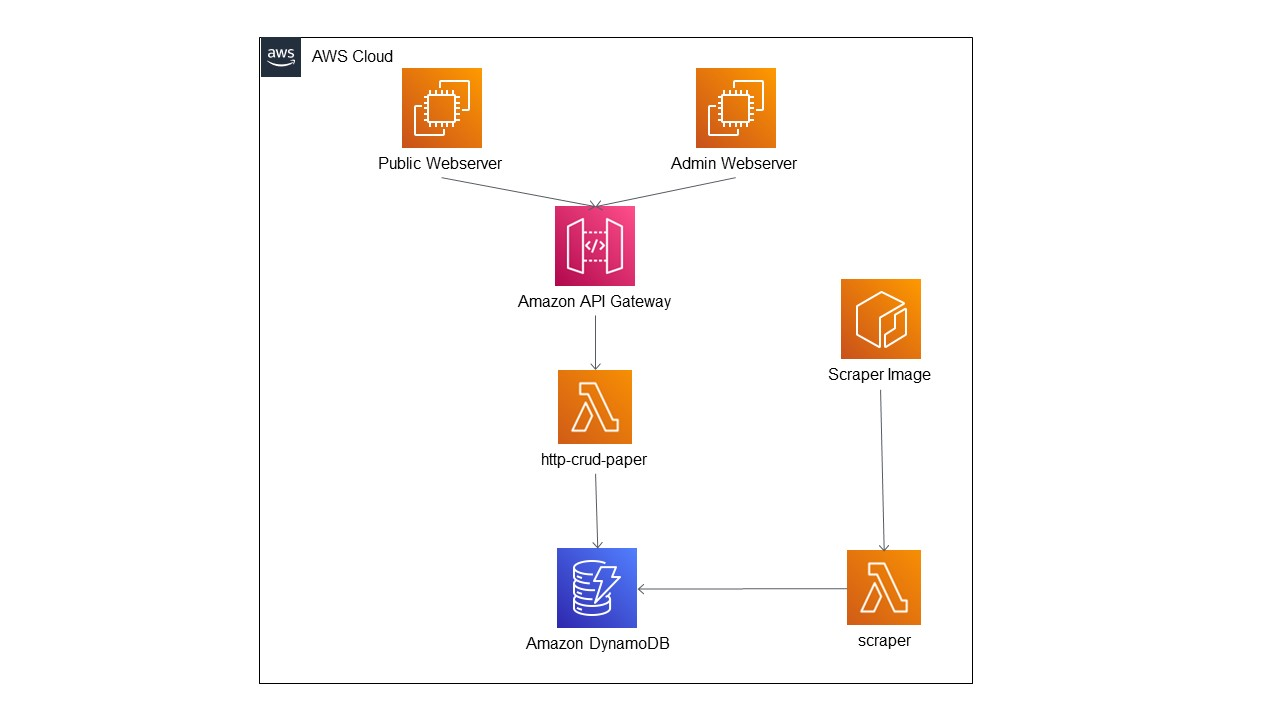
\includegraphics[width=0.8\textwidth]{../docs-assets/AWS architecture.jpg}
    \end{center} 
\end{figure}

% ec2 instances 
Each webserver is hosted on a customized EC2 instance. A key part of the design is splitting the two different user interactions - that of a paper viewer and paper administrator - onto separate virtual machines. The idea is that the traffic demands on either will almost certainly be different. For example, there are certainly more students than academics at regular universities. As such, we would expect the traffic on the user oriented webservers to be higher. Therefore, this separation of concerns allows more or less instances to be brought online in response to differential traffic/demand. This could be accomplished using a load balancer coupled with auto-scaling in the future. In essence, this separation makes it easy to tweak individual provisioning to match the demand. 
Furthermore, anticipating this extension, both EC2 instances use pm2 software installed to automatically run their respective webservers on restart. 

Each instance is also associated with an elastic IP. The idea here again relates to the load balancing with the operation of multiple instances where the elastic IPs can mask the failures of instances by instant remapping the address to other running instances. Furthermore, upon acquiring a domain name, this can ensure that the domain points to the instance(s).

% API
The API is provisioned using a combination of an API Gateway and a lambda function. The key idea here is running code only on demand. In this instance, the API Gateway service is always visible and able to be accessed. However, the lambda function only runs the code required to accomplish the request when the endpoint is triggered, thereby saving money.   

%Scrapers
The scrapers are provided through a Lambda function. A custom image is uploaded to an ECR repository that is then loaded by the Lambda function as its base image. This image is created through the use of Docker. However, this function is only able to be triggered manually from the console. In this way, the scrapers are only run when it makes sense to do so and only charged for exactly this time.

% Database
The database backend is provided by the DynamoDB service. This service greatly simplifies the backend logic since AWS takes care of all the particulars. Thus, all that is required is the correct triggering of the provided API. 

\subsection{Data Model}
The database consists of a single collection named papers.

\begin{figure}
    \caption{Paper collection data model.}
    \label{fig: paper_data_model}
    \begin{center}
        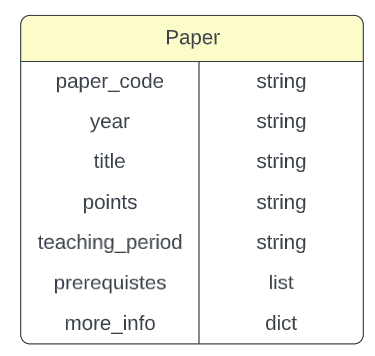
\includegraphics[width=0.2\textwidth]{../docs-assets/paper_erd.PNG}
    \end{center}
\end{figure}

Note that the paper objects can refer to other paper objects. In this case, I opted for a NoSQL database because it more easily links with the graph structure I wanted to accomplish with the paper structures. While some recent RDBMSs do offer tree structures without significant slowdown, I determined that in this case, with the small workload I am anticipating, it is simply easier and less logically intense to use a simple document oriented NoSQL database.

\section{Lifecycles}

This details the application lifecycle. Note that separate instructions are provided for starting the application from the AWS learner lab. 

\subsection{Initial setup}

These steps detail the inital configurations required for first time setup.

\subsubsection{Backend Setup}

First we need to initialize the backend DynamoDB database. To do this, first navigate to $https://console.aws.amazon.com/dynamodb/$ to bring up the DynamoDB interface. From here, we then create a table named $paper_table$ with primary partition key $id$. Note that on once created, successive restarts of the AWS learner lab will restart the table automatically, so no further effort is required. 

\subsubsection{Webserver setup}

To setup the webservers we first navigate to the EC2 console at $https://us-east-1.console.aws.amazon.com/ec2/$ and select $launch instance$. First, choose the Amazon Linux 2 AMI with a t2.micro instance and a specified key pair. Then create a new security group that allows SSH traffic from $myIP$, HTTP, HTTPS and custom TCP connections on port 3000 for IPv4 and IPv6 from the internet. This ensures that web users can connect to the React webserver that runs on port 3000. Note that the $myIP$ reference will have to be updated periodically. 

Then we assign elastic IPs to the instances using the $Elastic IPs$ tab under $Network and Security$. To do this, simply select $Allocate Elastic IP address$ and assign each webserver to different Elastic IPs.

Now connect to the webservers by following the instructions under $connect to instance$ and run the following sequence of commands. 

\begin{enumerate}
    \item $sudo yum install git -y$ to install git
    \item $git clone https://github.com/hadwi537/UniGuideOnline.git$ to install the application files (using a private access token if required).
    \item Setup Node.js runtime
    \begin{enumerate}
        \item $curl -o- https://raw.githubusercontent.com/nvm-sh/nvm/v0.34.0/install.sh | bash$
        \item $. ~/.nvm/nvm.sh$
        \item $nvm install --lts$
        \item $node -e "console.log('Running Node.js ' + process.version)$ to verify installation.
    \end{enumerate}
\end{enumerate}

Now navigate to the root directory of the one of the webservers (public-webserver or admin-webserver) and run $npm install$.

The respective app will now be available on localhost:3000 and from the given elastic IP at $http://<elastic-ip>:3000$.

We now configure PM2 to automatically start the webservers and leave them running when the terminal is closed through the following commands.

\begin{enumerate}
    \item $npm install pm2@latest -g$
    \item $npm install -g serve$
    \item $npm run build$ (from the root directory of a webserver)
    \item $pm2 serve build 3000 --spa$
    \item copy and paste the output of $pm2 startup$ and run it.

\end{enumerate}
    
\subsubsection{API Setup}

First setup the lambda function by navigating to $https://console.aws.amazon.com/lambda$ and select $create function$. Let the function name be $crud-paper-function$, assign the exectuion role to $LabRole$ and ensure that the LabRole has the $Simple microservice permissions$.

Then copy and paste the index.js code in $lambda/index.js$ into the code on the management console and press deploy.

We then create an HTTP API using API gateway. Navigate to the API Gateway console at $https://us-east-1.console.aws.amazon.com/apigateway/$ and choose $create API$ using the HTTP API blueprint. Use $crud-paper-api$ as the name and skip the remaming steps to create the API. 

Now select this API and choose $Routes$ under $Develop$. For each route we defined in the lambda function, we add that route with the specified method. In this case: 

\begin{itemize}
    \item $GET /papers/{id} $
    \item $GET /papers/$
    \item $PUT /items$
    \item $DELETE /items/{id}$
\end{itemize}

Now select $Integrations$ and assign the lambda api created in the previous step to every route.

\subsubsection{Scraper setup}

First create an ECR repository from the console $https://us-east-1.console.aws.amazon.com/ecr/$ and name it scraper-2. To create the image use $docker build -t scraper .$ from the scraper directory. 

Then, navigate to the lambda function console and create a lambda function in the usual way. Execept, in this case, choose the base image as the image residing in the ECR repository. Then login through docker using $docker login -u AWS -p \$(aws ecr get-login-password --region us-east-1) 426627924972.dkr.ecr.us-east-1.amazonaws.com$, tag the image with $docker tag scraper:latest 426627924972.dkr.ecr.us-east-1.amazonaws.com/scraper-2$ and push it to ECR using $docker push 426627924972.dkr.ecr.us-east-1.amazonaws.com/scraper-2$. 
The create a Lambda function in the usual way from the console except that we select the $Container image$ option and select the uploaded image using its image URI. For example $426627924972.dkr.ecr.us-east-1.amazonaws.com/scraper-2:latest$ as it will always be the latest.

\subsection{Development and Deployment}

As stated earlier, the DynamoDB requires no further modification. Unless, a more compute intensive option is desired.

In general, I personally recommend making changes locally. For example, since we are using a React web framework, the webservers can be run from the command line using npm-start where changes to the code can be instantly applied by simply saving the project. 

\subsubsection{Webservers}

Assuming that changes have been made and pushed to remote, connect to the ec2 instance hosting the changed webserver. Then, perform the following steps.

\begin{enumerate}
    \item $git pull$
    \item $npm install$ from the root directory of the modified webserver.
    \item $npm run build$,
    \item $pm2 stop all$
    \item $pm2 serve build 3000 --spa$ 
    \item copy and paste the output of $pm2 startup$ and run it in the terminal.
\end{enumerate}

\subsubsection{API}

For updating the lambda function, navigate to the Lambda function console and copy and paste in the changes.

New API routes can be created by following the steps detailed in the setup section.

\subsubsection{Scraper}

Upon making a change simply rebuild and push the image to ECR using the steps described above. Then update the Lambda function image by using the $Deploy new image button$ and selecting the latest image.

\section{Estimated costs of cloud services}
% estimation of running costs
The estimated running costs are detailed below.

% idle
In idle conditions, the monthly cost is about $31.55$

% with light use
With light use, the monthly cost is about $41.38$ where the majority of the cost comes from the DynamoDB database.

\section{User Interaction}

The application is designed to be used by a client through a web interface. Users can either view paper data visualizations or create papers through the website interface. 


\section{Development story}

% terraform 
I initially attempted to use terraform in order to automatically provision my resourecs as I figured that this would ultimately be an easier way to work.
However, I was defeated by the IAM role that had to be assigned to lambda function resources would lead t me being either locked out of certain functionality (i.e I couldn't see my functions on the AWS GUI) and to terraform destroy failing because the IAM user couldn't be deleted with it.

%ec2 
Creating the ec2 instances was relatively smooth. As with the last assignment, I used the React framework mostly because I was now familiar with its operation. While I decided to have a static webserver. It is reasonably easy to create a dynamic one using React so I felt this option left future development nicely open.
However, I did try and create a CI/CD pipeline to simplify the application lifecycle. However, AWS academy does not let you do this.

%dynamoDB
I then decided to use DynamoDB primarily because the previous app this is based off was setup to function with a NoSQL database. Furthermore, I found it a bit simpler to interact with from the context of a lambda function than the RDBMS offering.

%API
Clearly I was always going to need a nice way to interact with the different components. I decided to have a serverless function so that I didn't have to run another virtual machine which would be both expensive, slow and difficult to maintain (especially without CI/CD).

Finally, I decided to include the scrapers in the application after all. My initial thought was to again use serverless functions because, logically, it maps well to think of the scrapers like a function that gets executed at some time. Furthermore, it saves money compared to running EC2 instances.

% eventual outcome

\section{Future improvements}

% CI/CD
The first thing I would like to do would be to use CI/CD. This would allow changes to the code to be transferred to production in a structured and careful manner, saving the issue of having to manually pull from EC2 instances on code changes. However, this is not possible with learner lab so this would require a personal account.

% Authorization control/user accounts for managing data
On the website end, I would like to implement the creation of user accounts such that the privileges for interacting with resources (such as papers) can be restricted, so only their owners can interact with them. Therefore, it follows that I would also like to add some href system such that both webserver types are connected through an authentication dialog. 

% cloud front network
In order to allow this application to properly scale, I would like to implement a CDN and load balancing services in order to balance the demands of user interaction through modifying the number of webserver instances as this would greatly increase the reliability of the application. 

% terraform
After these changes, I believe that complexity would grow such that it may justify the use of terraform. However, the learner lab does not support this functionality as lambda functions require roles which cannot be cleanly accomplished with terraform as it causes certain lifecycle elements to fail. 

\end{document}